\documentclass[twocolumn,a4paper]{article}
\usepackage{fontspec}   %加這個就可以設定字體
\usepackage{xeCJK}       %讓中英文字體分開設置
\usepackage{indentfirst}
\usepackage{listings}
\usepackage[newfloat]{minted}
\usepackage{float}
\usepackage{graphicx}
\usepackage{caption}
\usepackage{fancyhdr}
\usepackage{hyperref}
\usepackage{amsmath}
\usepackage{multirow}
\usepackage[dvipsnames]{xcolor}
\usepackage{graphicx}
\usepackage{tabularx}
\usepackage{booktabs}
\usepackage{caption}
\usepackage{subcaption}
\usepackage{pifont}
\usepackage{amssymb}


\usepackage{pdftexcmds}
\usepackage{catchfile}
\usepackage{ifluatex}
\usepackage{ifplatform}

\usepackage[breakable, listings, skins, minted]{tcolorbox}
\usepackage{etoolbox}
\setminted{fontsize=\footnotesize}
\renewtcblisting{minted}{%
    listing engine=minted,
    minted language=python,
    listing only,
    breakable,
    enhanced,
    minted options = {
        linenos, 
        breaklines=true, 
        breakbefore=., 
        % fontsize=\footnotesize, 
        numbersep=2mm
    },
    overlay={%
        \begin{tcbclipinterior}
            \fill[gray!25] (frame.south west) rectangle ([xshift=4mm]frame.north west);
        \end{tcbclipinterior}
    }   
}

\usepackage[
top=1.5cm,
bottom=0.75cm,
left=1.5cm,
right=1.5cm,
includehead,includefoot,
heightrounded, % to avoid spurious underfull messages
]{geometry} 

\newenvironment{code}{\captionsetup{type=listing}}{}
\SetupFloatingEnvironment{listing}{name=Code}



\title{Visual Recognition using Deep Learning - HW1}
\author{110550088 李杰穎}
\date{\today}


\setCJKmainfont{Noto Serif TC}



\ifwindows
\setmonofont[Mapping=tex-text]{Consolas}
\fi

\XeTeXlinebreaklocale "zh"             %這兩行一定要加,中文才能自動換行
\XeTeXlinebreakskip = 0pt plus 1pt     %這兩行一定要加,中文才能自動換行

\newcommand*{\dif}{\mathop{}\!\mathrm{d}}


%\setlength{\parindent}{0em}
%\setlength{\parskip}{2em}
%\renewcommand{\baselinestretch}{1.25}
%\setlength{\droptitle}{-7.5em}   % This is your set screw
%\setlength{\columnsep}{2em}

\begin{document}

\maketitle
\section{Introduction}

This homework addresses the challenging task of fine-grained image classification across 100 diverse classes, encompassing insects, plants, and birds. The dataset presents several key challenges: (1) complex scenes with mixed foreground and background elements, (2) images containing multiple objects of interest, and (3) significant intra-class variation, such as classes containing both butterflies and their caterpillar forms. The dataset comprises 21,024 images for training and validation, with an additional 2,344 test images for evaluation.

To tackle these challenges, I employ ResNeSt\cite{zhang2022resnest} as the backbone architecture, which enhances the original ResNet\cite{he2016deep} design with Split-Attention blocks for improved feature representation. For robust training, I employ a comprehensive augmentation strategy combining \texttt{TrivialAugmentWide}\cite{muller2021trivialaugment}, Mixup\cite{zhang2018mixup}, and CutMix\cite{yun2019cutmix} techniques. This multi-faceted approach to data augmentation addresses the various object scales, positions, and contextual variations present in the dataset.

Additionally, I implement test-time augmentation to further improve prediction accuracy by averaging predictions across multiple transformed versions of each test image. This comprehensive approach yields excellent results, achieving 93\% validation accuracy and 97\% testing accuracy. The complete implementation, including training configurations and evaluation scripts, is available in the project repository at \url{https://github.com/jayin92/NYCU-VRDL-HW1}.

\section{Method}

In this homework, I mainly focus on utilizing different data argumentation techniques, thus, I directly employ off-the-shelf model architectures without modifying them except the output number of classes.

\subsection{Model Architectures}
\textbf{ResNet}\cite{he2016deep} is the ground-breaking CNN architecture that first utilized residual connections to mitigate the gradient vanishing problem when training very deep neural networks. By introducing skip connections that allow gradients to flow more easily through the network, ResNet enabled the successful training of networks with hundreds of layers. The key insight behind ResNet is that it's easier to optimize the residual mapping than the original mapping. This innovation led to significant performance improvements on ImageNet classification and inspired numerous subsequent architectures. ResNet serves as the base model in this homework.

\textbf{ResNeXt}\cite{xie2017aggregated} extends the ResNet architecture by introducing ``cardinality'' as a new dimension alongside width and depth. Instead of simply making networks wider or deeper, ResNeXt aggregates a set of transformations with the same topology using grouped convolutions. This approach increases model capacity without significantly increasing computational complexity. The "split-transform-merge" strategy allows ResNeXt to achieve better performance than ResNet on various vision tasks while maintaining similar parameter counts, demonstrating that carefully designed aggregated transformations can be more effective than increased width or depth alone.

\textbf{ResNeSt}\cite{zhang2022resnest} builds upon both ResNet and ResNeXt by incorporating Split-Attention blocks within the bottleneck structure. These blocks enable feature map attention across different feature groups, allowing the network to selectively emphasize informative features. ResNeSt combines cross-channel attention with spatial attention mechanisms, resulting in improved feature representation. This architecture maintains computational efficiency while achieving state-of-the-art results across multiple computer vision tasks including image classification, object detection, and instance segmentation, making it a versatile backbone for various applications. We use ResNeSt-200 as the backbone model for this homework, use pre-trained from ImageNet classification.


\subsection{Data Augmentations}
\paragraph{TrivialAugment\cite{muller2021trivialaugment}.} In this homework, I employ a simple yet effective data augmentation technique called TrivialAugment\cite{muller2021trivialaugment} to enhance the training data. TrivialAugment operates by randomly sampling one augmentation operation $a$ from a predefined set $\mathcal{A}$ and a discrete strength parameter $s$ that controls the intensity of image distortion. The set $\mathcal{A}$ encompasses various transformations including translation, rotation, brightness adjustment, color jittering, and more. Despite its simplicity, TrivialAugment has been empirically shown to outperform many sophisticated automated data augmentation methods, offering a good balance between implementation complexity and performance improvement.

\paragraph{Mixup\cite{zhang2017mixup}.} To further enhance model generalization, we implement Mixup\cite{zhang2017mixup} augmentation, which creates virtual training examples by linearly interpolating between pairs of images and their corresponding labels. Specifically, for two randomly selected training examples $(x_i, y_i)$ and $(x_j, y_j)$, Mixup generates a new training sample $(\tilde{x}, \tilde{y})$ where $\tilde{x} = \lambda x_i + (1-\lambda) x_j$ and $\tilde{y} = \lambda y_i + (1-\lambda) y_j$, with $\lambda \sim \text{Beta}(\alpha, \alpha)$ and $\alpha$ being a hyperparameter controlling the interpolation strength. This technique encourages the model to behave linearly in-between training examples, reduces memorization of noisy labels, and improves robustness to adversarial examples. In our implementation, Mixup works with other augmentation techniques to regularize the model and promote smoother decision boundaries.

\paragraph{CutMix\cite{yun2019cutmix}.} We discover that in this dataset, the target objects often have very distinct features and mixed spatial distributions. Thus, in order to increase model robustness and generalization capabilities, we implement CutMix\cite{yun2019cutmix} augmentation. CutMix works by randomly cutting rectangular regions from one training image and pasting them onto another, while simultaneously mixing the labels proportionally to the area of the patch. This technique encourages the model to focus on both primary and secondary features within images, reduces over-reliance on specific image regions, and enhances localization capability. Our experiments show that incorporating CutMix significantly improves classification accuracy, particularly for classes with similar features or when objects appear in various contexts within the dataset.

\paragraph{Test-time Data Augmentation.} As mentioned earlier, we found that images in this dataset often exhibit variations in scale, orientation, and object location. To compensate for these variations and improve classification accuracy, we employ test-time augmentation (TTA) during inference. Specifically, we apply 11 different transformations to each test image, including various scaling factors, horizontal flips, and 5-way cropping (top-left, top-right, center, bottom-left, and bottom-right). For each transformed version of the image, we obtain a prediction probability distribution over all classes. The final prediction is determined by averaging these probability distributions and selecting the class with the highest average probability. This ensemble approach enhances model performance by reducing the impact of spatial variations and providing more robust predictions.


\paragraph{Data argumentation pipeline.} We provide the full data argumentation pipeline written in PyTorch:

\begin{code}
\begin{minted}
train_transform = transforms.Compose([
    transforms.RandomResizedCrop(args.image_size, scale=(0.6, 1.0)),
    transforms.RandomHorizontalFlip(),
    autoaugment.TrivialAugmentWide(),
    transforms.ToTensor(),
    transforms.Normalize([0.485, 0.456, 0.406], [0.229, 0.224, 0.225]),
    transforms.RandomErasing(p=0.3, scale=(0.02, 0.33), ratio=(0.3, 3.3))
])
\end{minted}
\end{code}

We apply CutMix and MixUp in the training loop, with 25\% of probability performing CutMix, 25\% of probability performing MixUp and rest of 50\% probability don't apply any of these transformation.

\begin{code}
\begin{minted}
cutmix_transform = transforms_v2.CutMix(num_classes=num_classes)
mixup_transform = transforms_v2.MixUp(num_classes=num_classes)
# Randomly choose between CutMix and MixUp with equal probability
aug_transform = transforms_v2.RandomChoice([cutmix_transform, mixup_transform])
\end{minted}
\end{code}


\subsection{Hyperparameters}
\begin{itemize}
\item \textbf{Backbone:} ResNeSt-200 (68M)
\item \textbf{Batch size:} 64
\item \textbf{Image size:} 320
\item \textbf{Epochs:} 80
\item \textbf{Optimizer:} AdamW
\item \textbf{Learning rate:} 1e-4
\item \textbf{Weight decay:} 1e-4
\item \textbf{Learning rate scheduler:} OneCycle with cosine annealing
\end{itemize}

\section{Results}

\subsection{Training and Validation Performance}

The training process spanned 80 epochs using the ResNeSt-200 backbone with our comprehensive augmentation strategy. Figures~\ref{fig:trainloss} and \ref{fig:valloss} show the loss curves for training and validation respectively, while Figures~\ref{fig:trainacc} and \ref{fig:valacc} display the corresponding accuracy metrics.

The training loss exhibits a decrease during the initial epochs, followed by gradual stabilization. This training curve, despite the complexity of the dataset, indicates effective regularization from our multiple augmentation techniques (TrivialAugmentWide, Mixup, and CutMix).

The validation loss closely follows the training loss pattern but with slightly higher values, demonstrating good generalization without significant overfitting. The fluctuations observed are expected due to the diverse nature of the validation set and the probabilistic nature of our augmentation techniques. The validation accuracy reaches approximately 93\%, which confirms the model's ability to generalize well across the 100 diverse classes.

\begin{figure}[H]
\centering
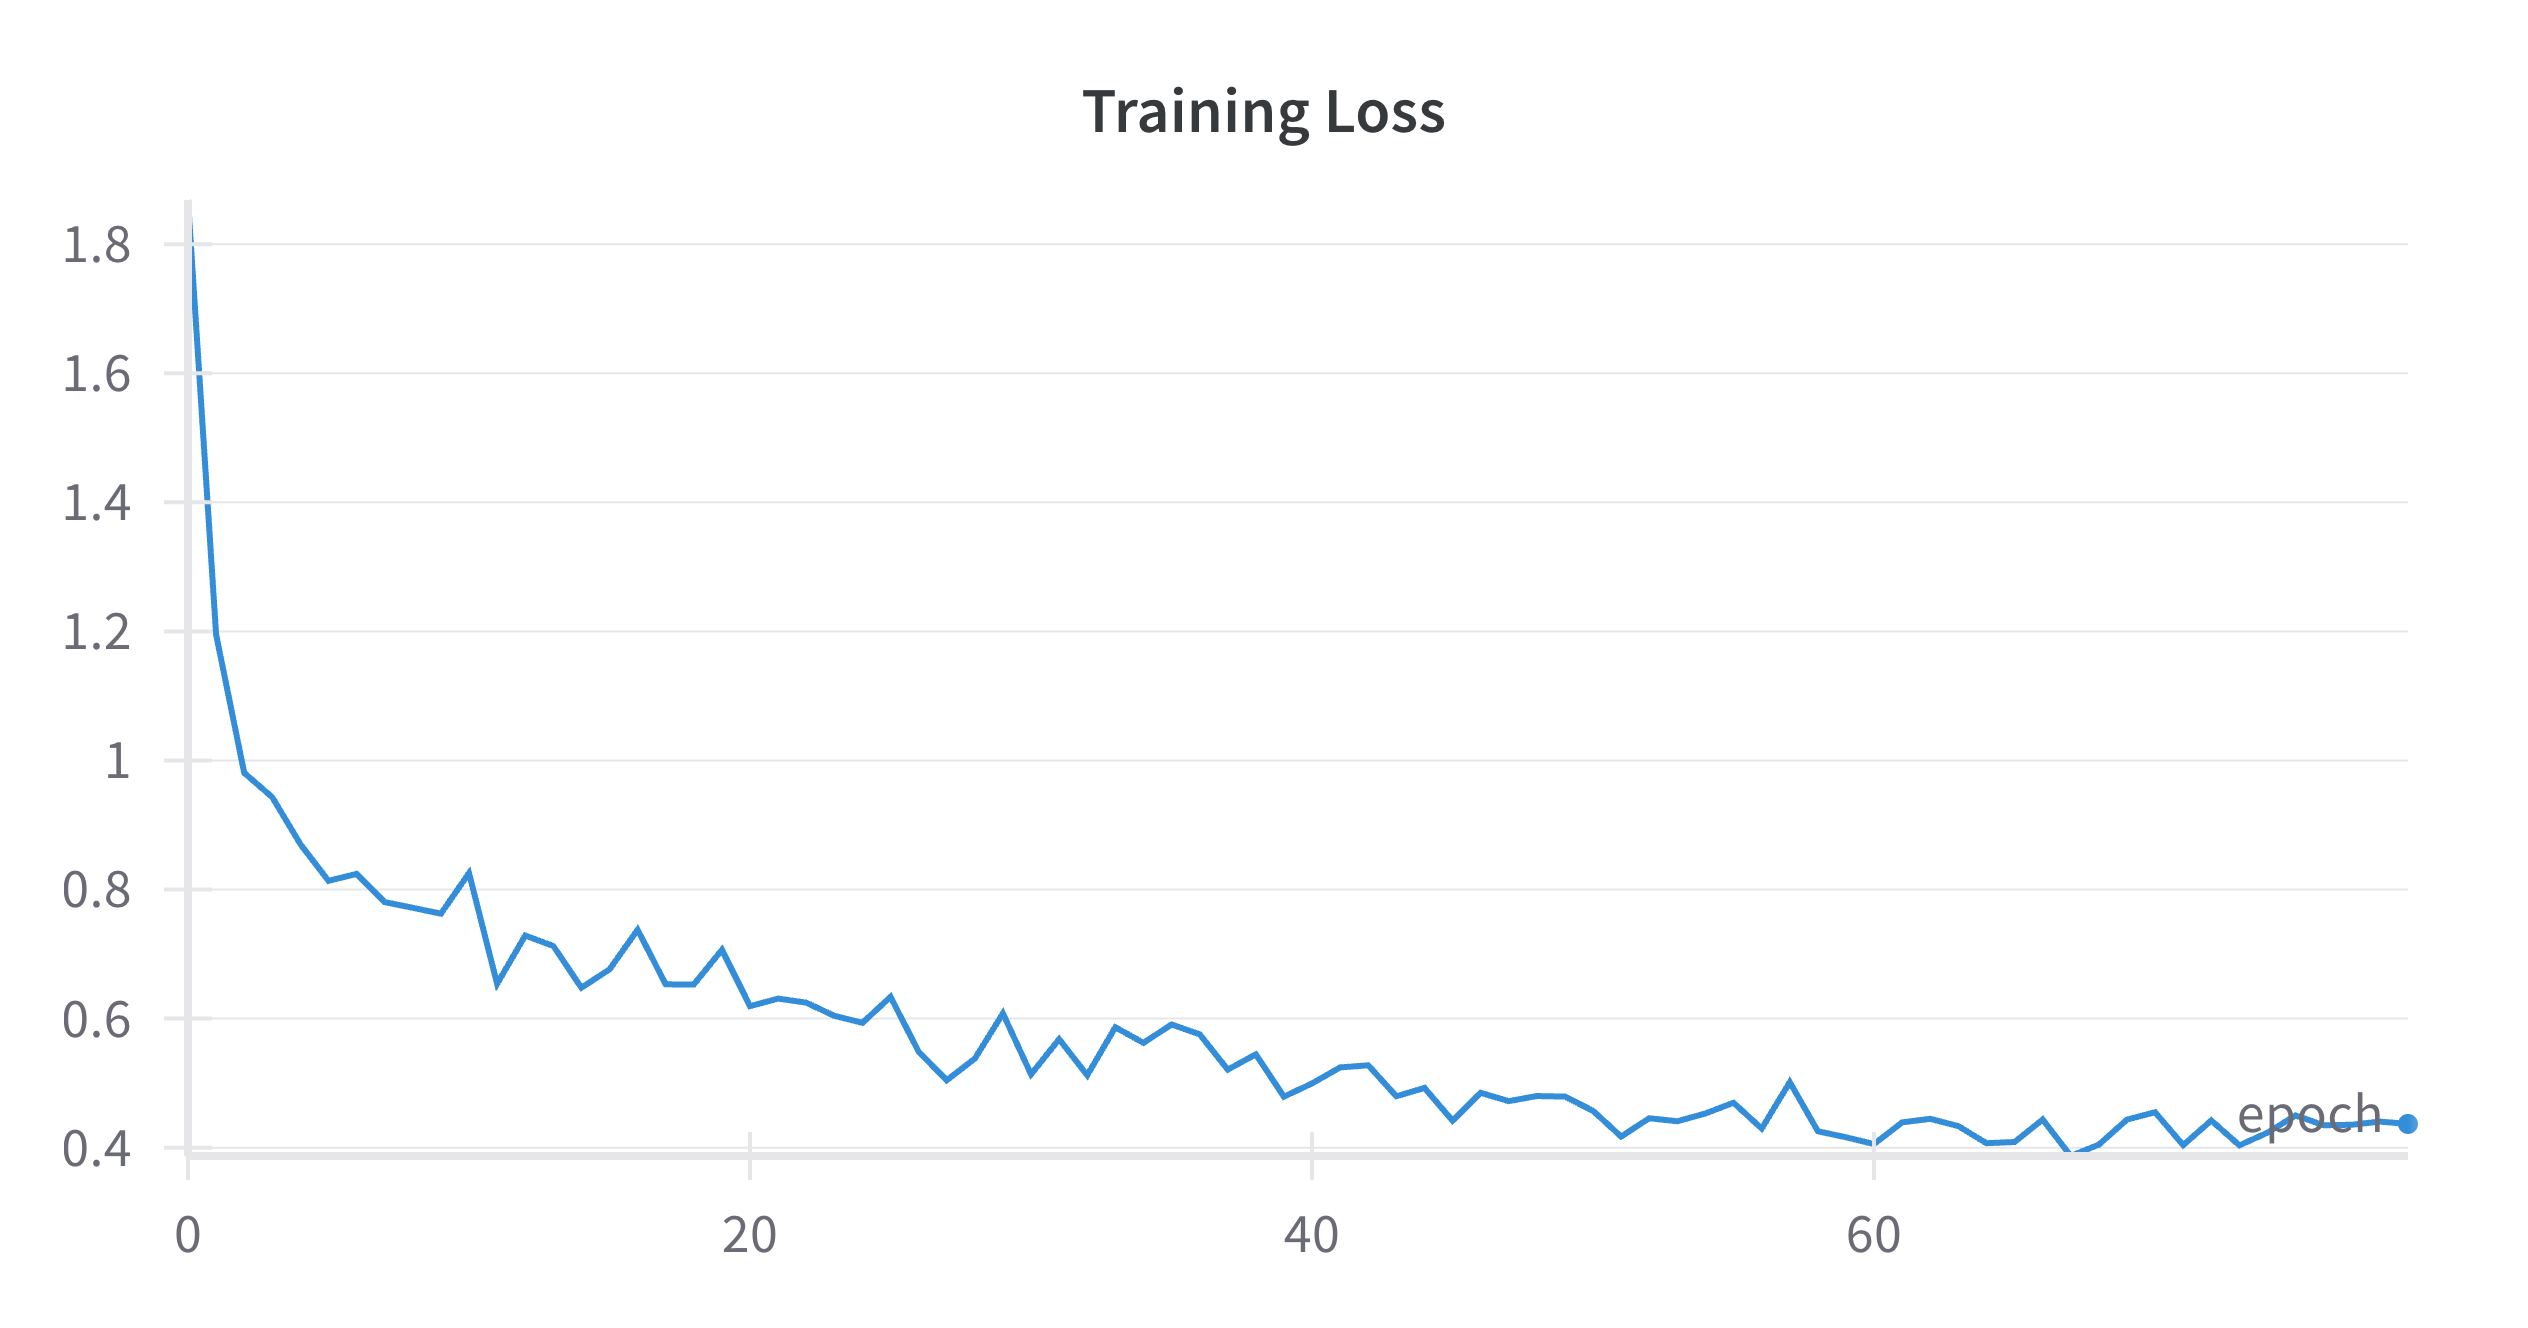
\includegraphics[width=0.95\linewidth]{figs/train_loss}
\caption{\textbf{Training loss progression over 80 epochs.}}
\label{fig:trainloss}
\end{figure}

\begin{figure}[H]
\centering
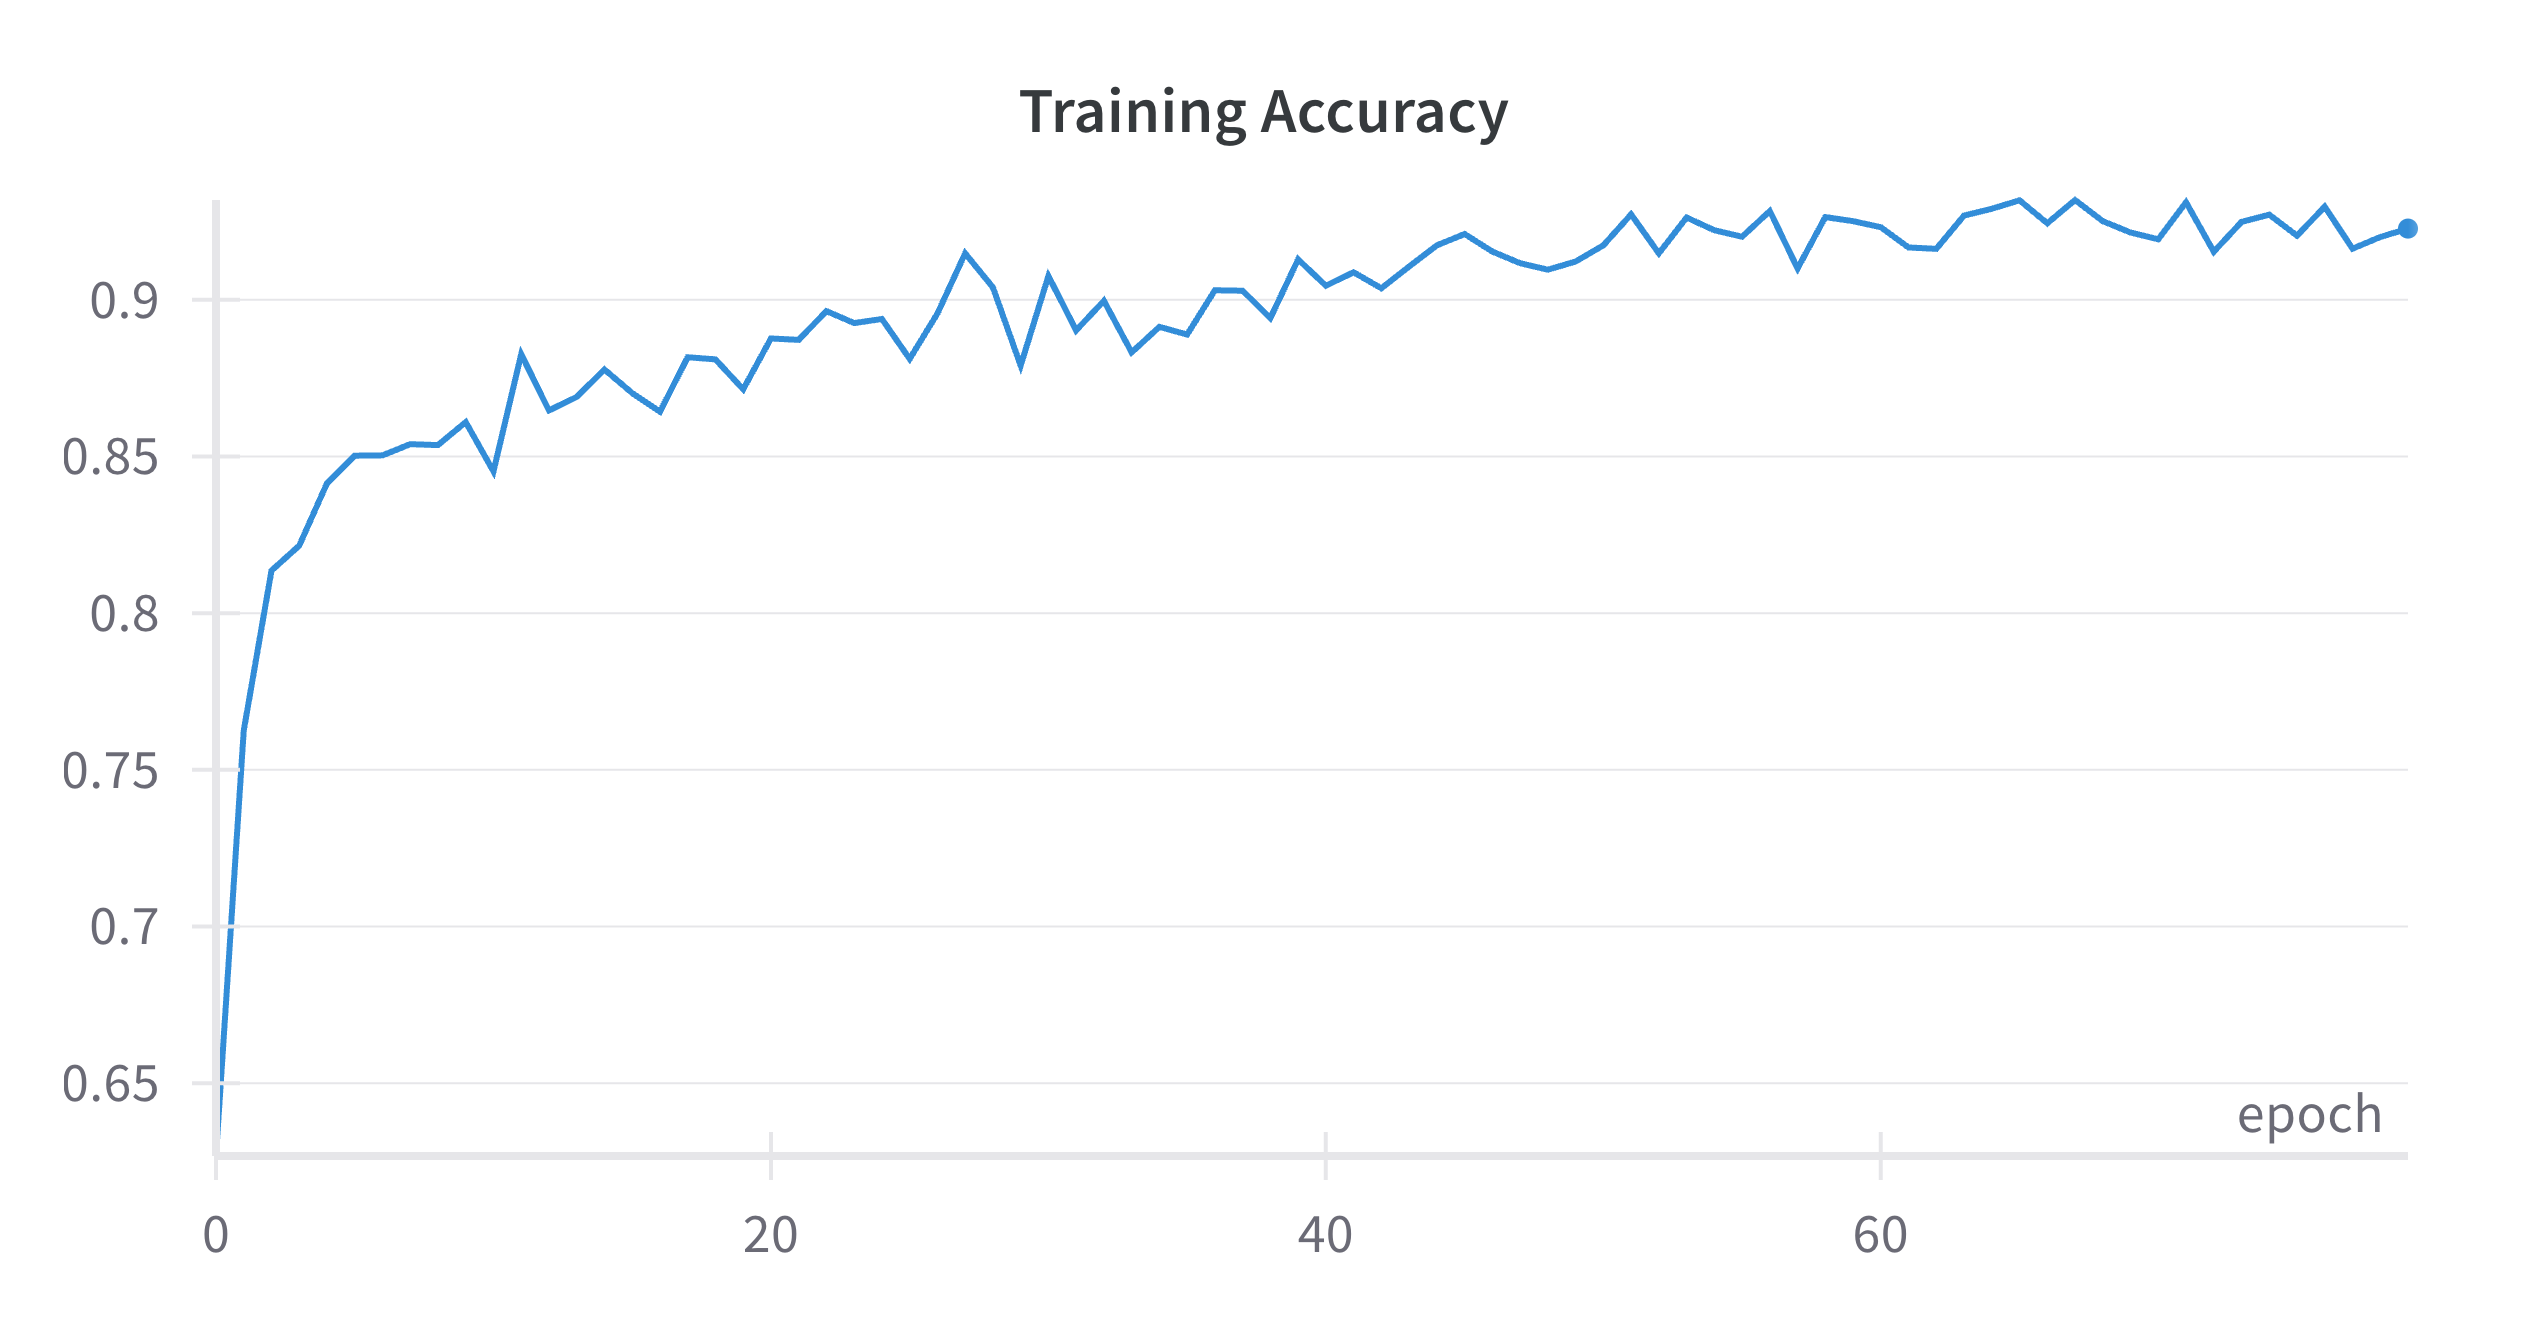
\includegraphics[width=0.95\linewidth]{figs/train_acc}
\caption{\textbf{Training accuracy progression over 80 epochs.}}
\label{fig:trainacc}
\end{figure}

\begin{figure}[H]
\centering
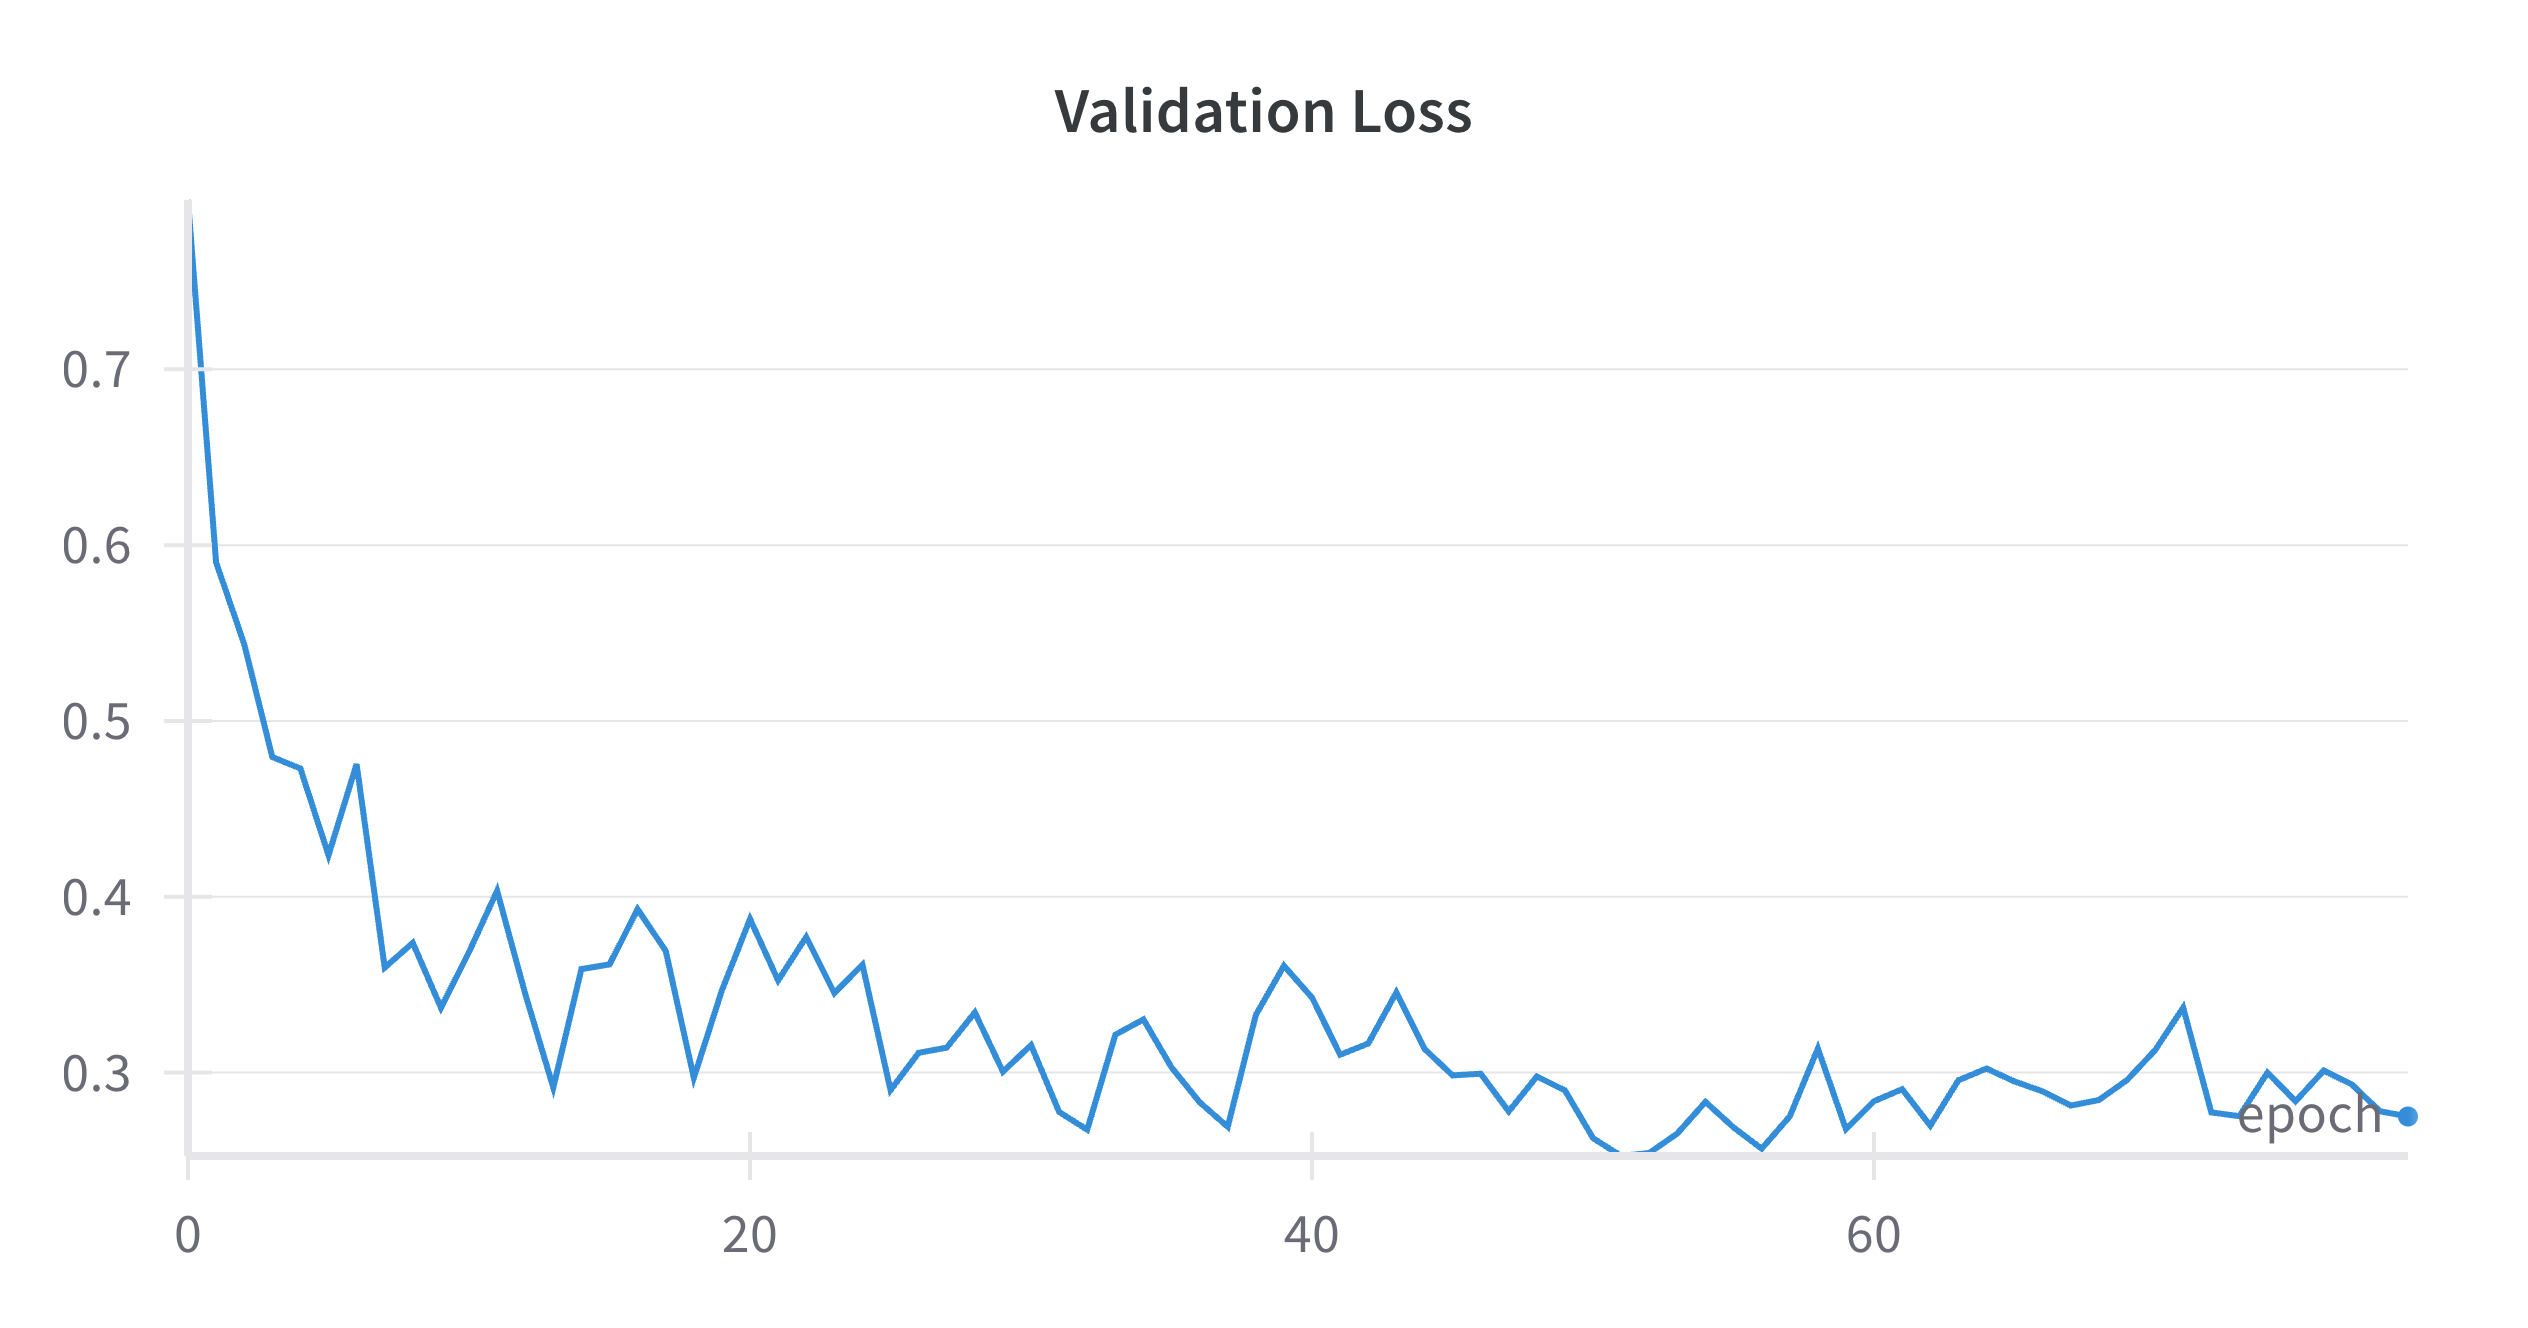
\includegraphics[width=0.95\linewidth]{figs/val_loss}
\caption{\textbf{Validation loss progression over 80 epochs.}}
\label{fig:valloss}
\end{figure}

\begin{figure}[H]
\centering
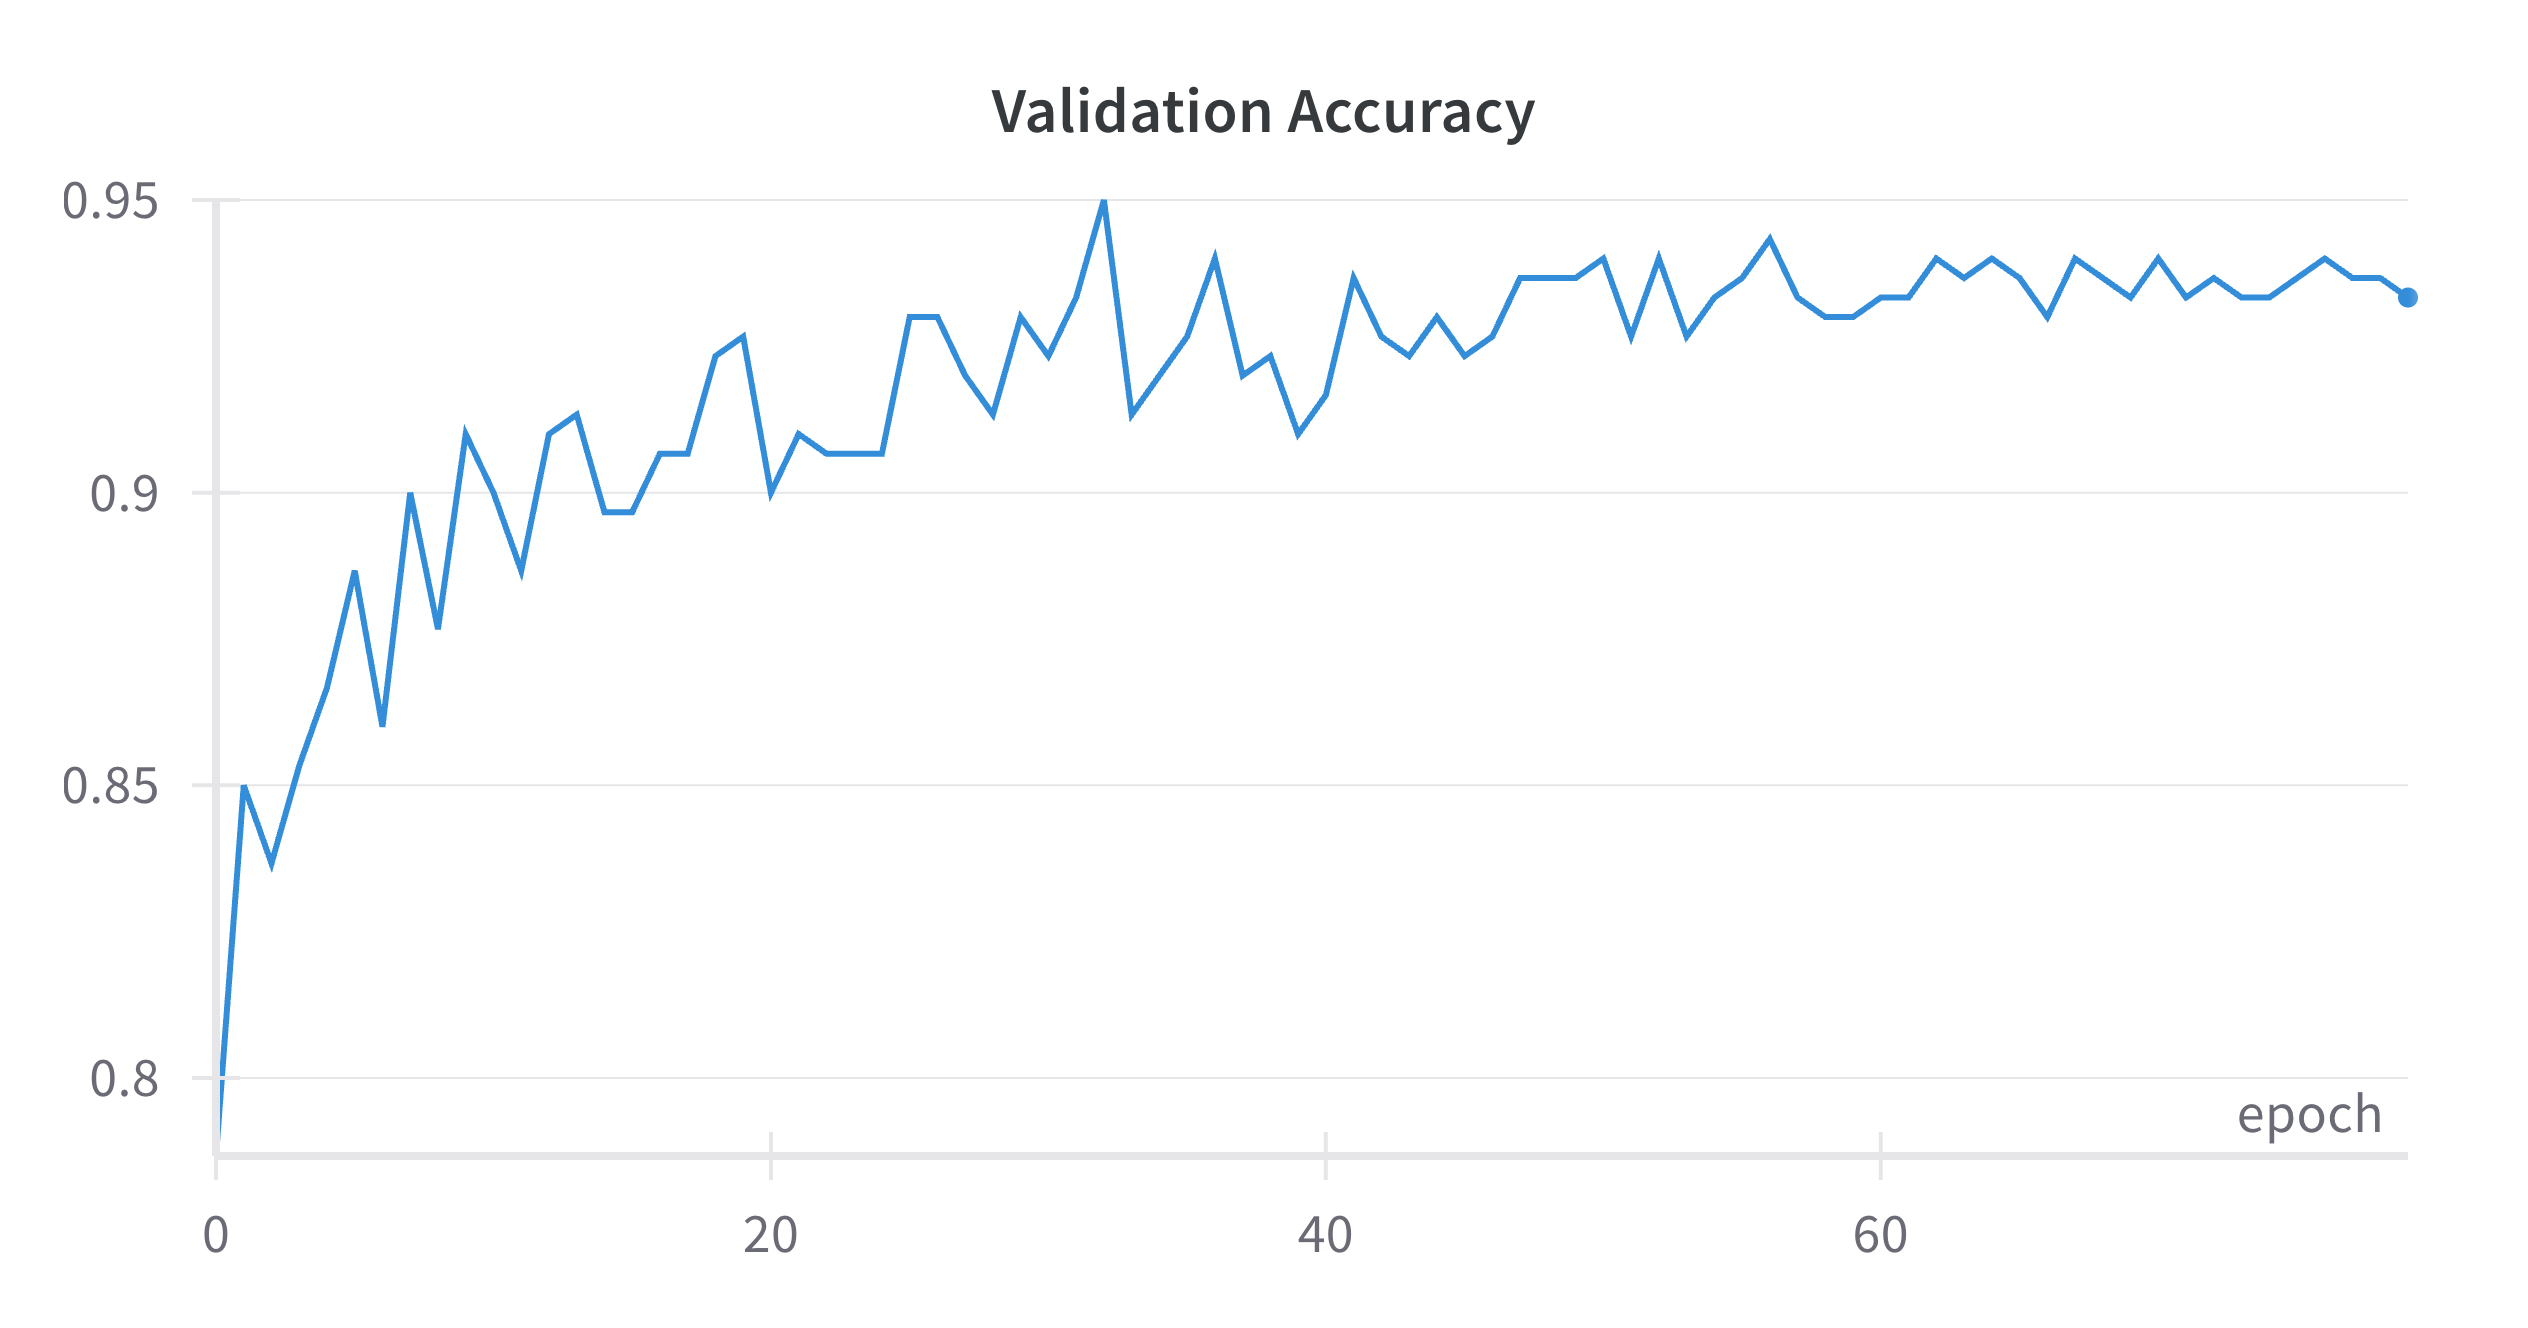
\includegraphics[width=0.95\linewidth]{figs/val_acc}
\caption{\textbf{Validation accuracy progression over 80 epochs.}}
\label{fig:valacc}
\end{figure}

\subsection{Competition Performance}

Our model achieved strong performance, as illustrated in Figure~\ref{fig:publicscore}. The final accuracy of 97\% on the public test set significantly surpasses the strong baseline of 92.3\%. This substantial improvement validates the effectiveness of our approach combining the ResNeSt-200 architecture with robust data augmentation and test-time augmentation.

\begin{figure}[H]
\centering
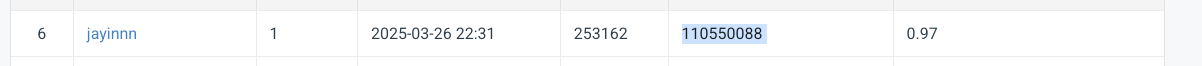
\includegraphics[width=0.95\linewidth]{figs/public_score}
\caption{\textbf{Model performance on the CodaBench public leaderboard.}}
\label{fig:publicscore}
\end{figure}

\subsection{Error Analysis}

Figure~\ref{fig:confusionmatrix} shows the confusion matrix for our model across all 100 classes. The strong diagonal pattern indicates high accuracy across most classes, with minimal misclassifications. The few off-diagonal elements represent challenging cases where classes share visual similarities or contain significant intra-class variations. Notable patterns include minor confusion between visually similar insect species and between different developmental stages of the same species (e.g., butterfly and caterpillar forms).

\begin{figure}[H]
\centering
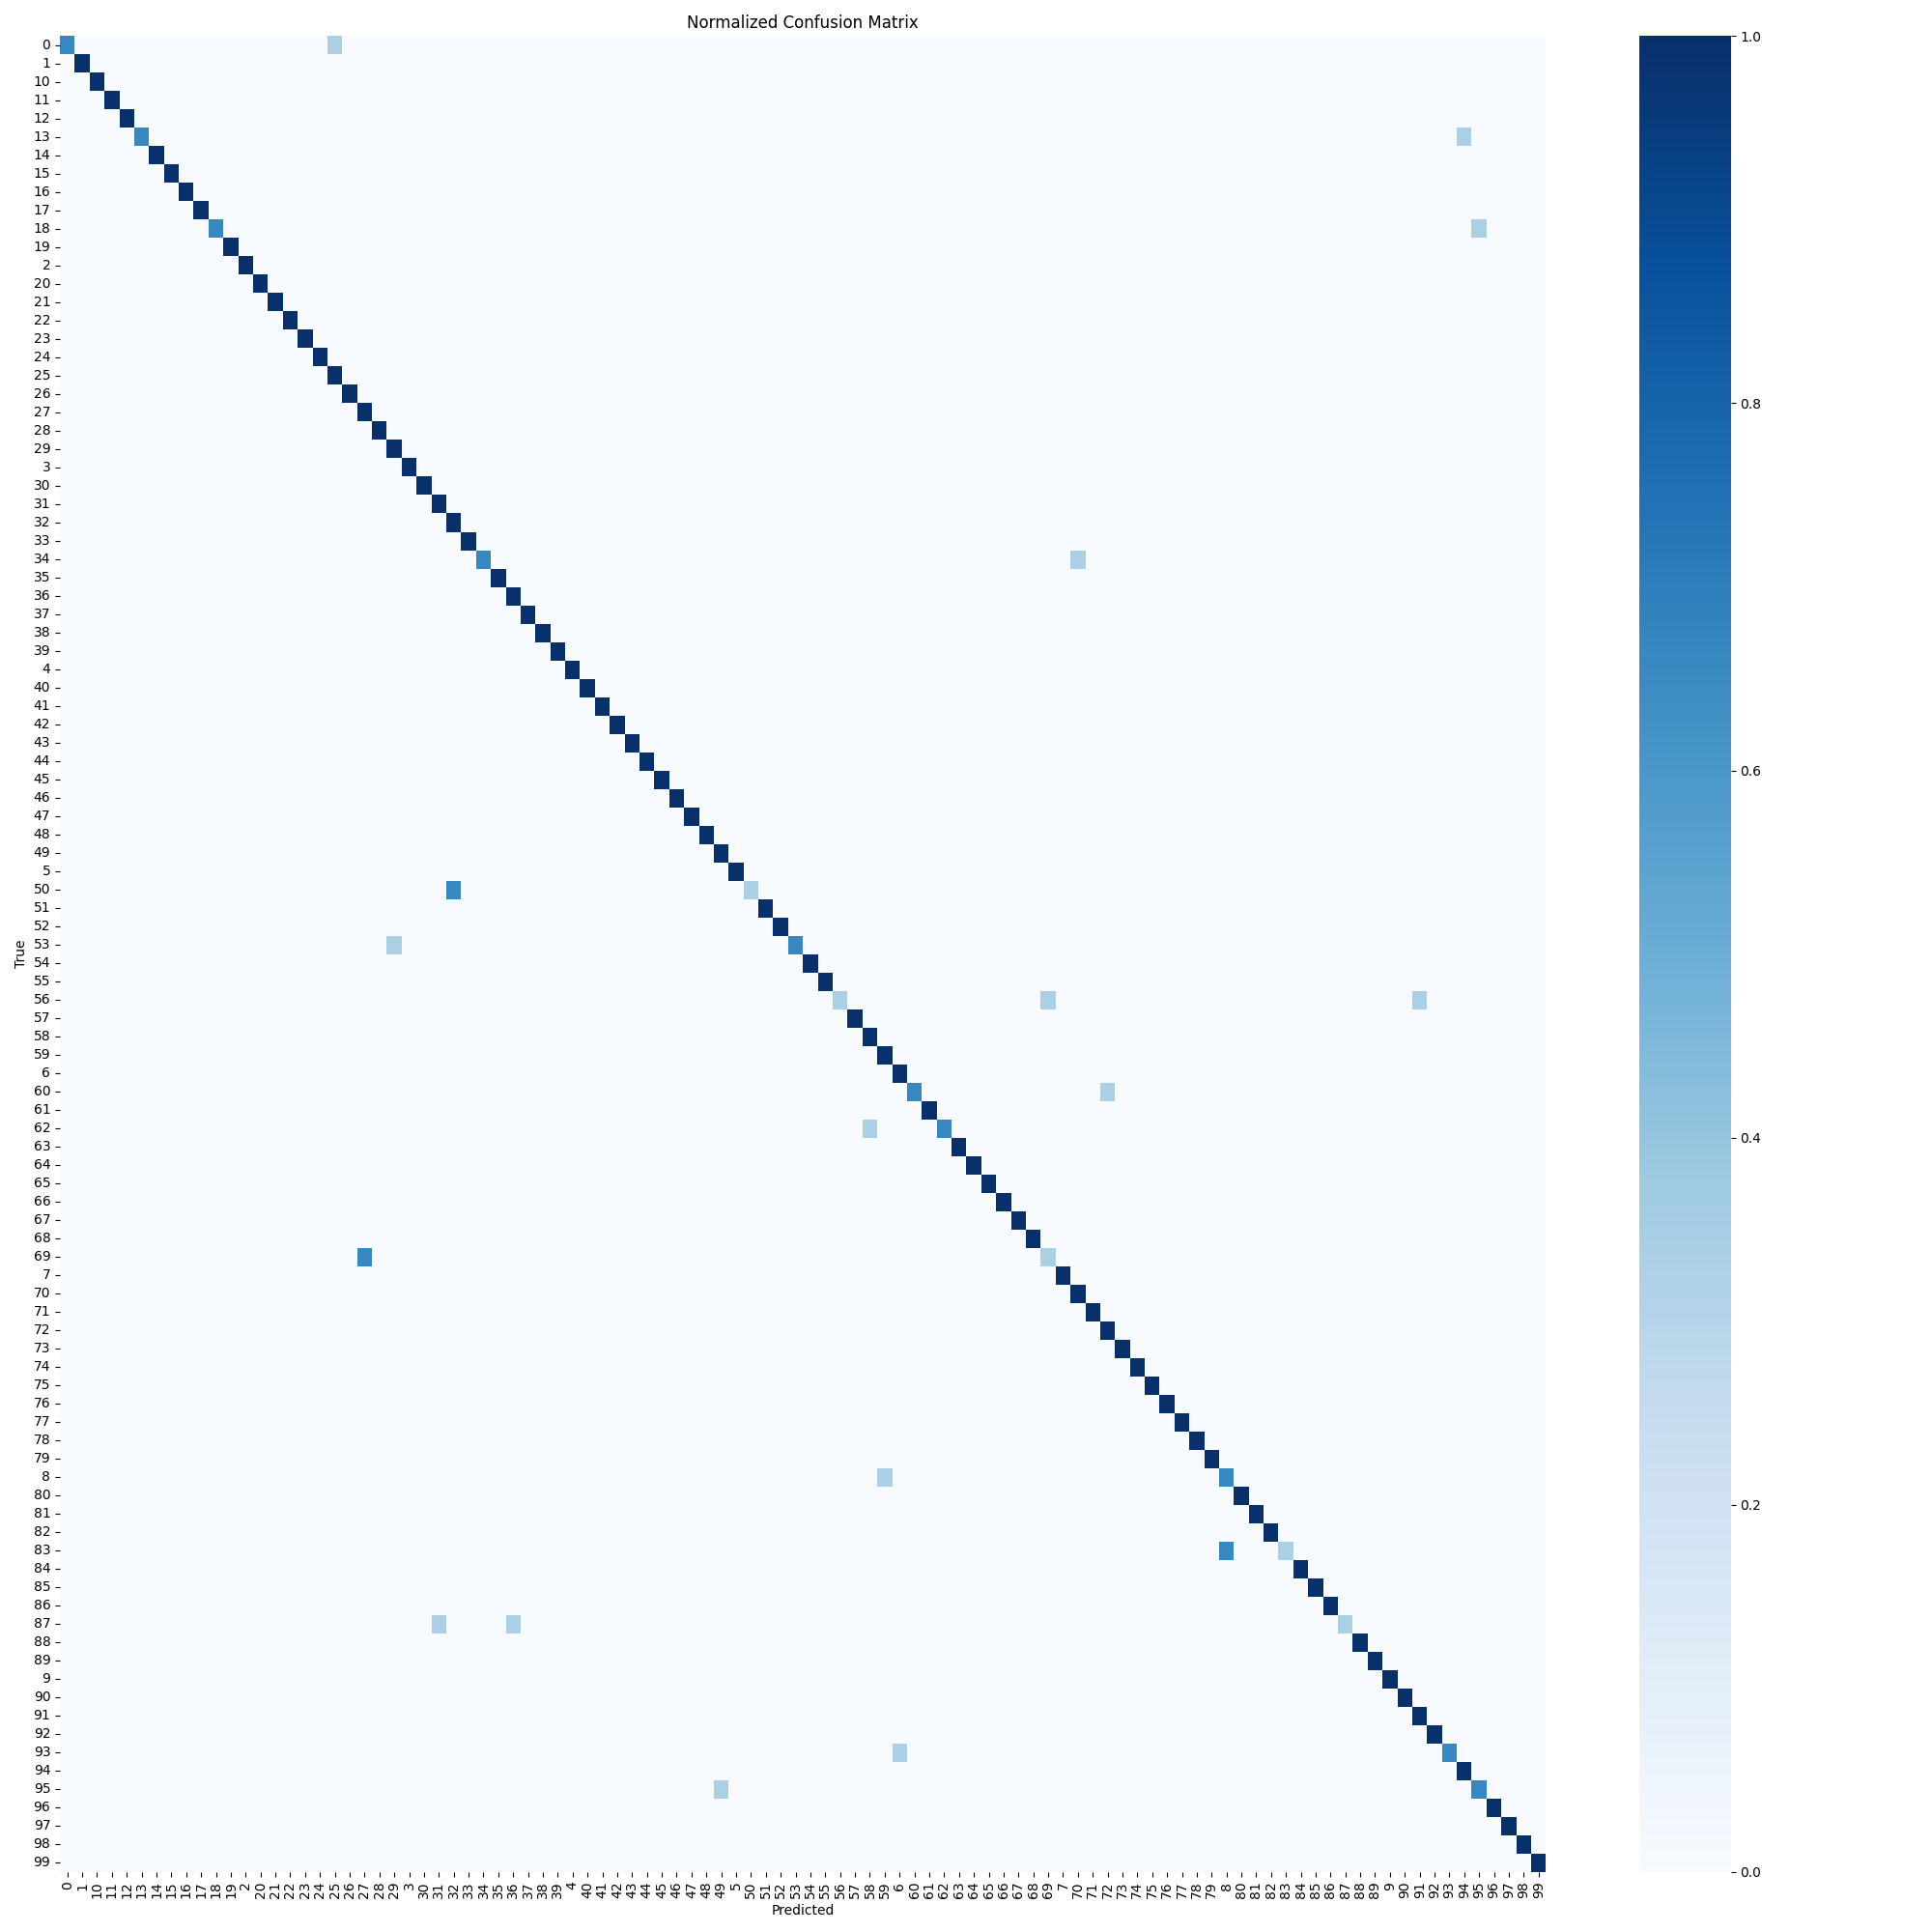
\includegraphics[width=0.95\linewidth]{figs/confusion_matrix}
\caption{\textbf{Confusion matrix across all 100 classes.}}
\label{fig:confusionmatrix}
\end{figure}

\subsection{Analysis and Discussion}

The experimental results demonstrate the effectiveness of our approach in addressing the fine-grained image classification challenge. The final model achieves 93\% validation accuracy and 97\% testing accuracy, significantly outperforming the baseline requirements.

Several key insights emerge from our results:

\begin{itemize}
\item The ResNeSt-200 backbone with Split-Attention blocks provides an effective architecture for capturing discriminative features across diverse object classes.

\item Our comprehensive data augmentation strategy proved crucial for handling the dataset's challenges:
  \begin{enumerate}
  \item TrivialAugmentWide helped address variations in object appearance and positioning
  \item Mixup improved model generalization and reduced overfitting
  \item CutMix enhanced the model's ability to focus on both primary and contextual features
  \end{enumerate}

\item Test-time augmentation provided a significant boost to final accuracy, demonstrating the importance of considering multiple views of test images for robust prediction.

\item The confusion matrix reveals that remaining misclassifications primarily occur between visually similar classes or between different developmental stages of the same species, which represent inherently challenging cases even for human experts.
\end{itemize}

These results highlight the importance of combining an appropriate model architecture with targeted data augmentation techniques for fine-grained image classification tasks. The approach demonstrates strong generalization capability across the 100 diverse classes while maintaining computational efficiency within the parameter budget constraints (ResNeSt-200 with 68M parameters, well below the 100M limit).


\bibliographystyle{plain}
\bibliography{main}


\end{document}